% Created 2021-02-25 Thu 21:58
% Intended LaTeX compiler: pdflatex
\documentclass[presentation]{beamer}
\usepackage[utf8]{inputenc}
\usepackage[T1]{fontenc}
\usepackage{graphicx}
\usepackage{grffile}
\usepackage{longtable}
\usepackage{wrapfig}
\usepackage{rotating}
\usepackage[normalem]{ulem}
\usepackage{amsmath}
\usepackage{textcomp}
\usepackage{amssymb}
\usepackage{capt-of}
\usepackage{hyperref}
\usepackage{minted}
\usepackage[utf8]{inputenc}
\usepackage{color}
\usetheme[height=7mm]{Rochester}
\setbeamertemplate{footline}[frame number]
\usecolortheme[accent=red, light]{solarized}
\setbeamercolor{frametitle}{bg=solarizedRebase02,fg=solarizedAccent}
\setbeamercolor{author in head/foot}{bg=solarizedRebase02,fg=solarizedRebase01}
\setbeamercolor{title in head/foot}{bg=solarizedRebase02,fg=solarizedRebase01}
\setbeamercolor{block title}{bg=solarizedRebase0,fg=solarizedRebase02}
\setbeamercolor{block body}{bg=solarizedRebase02,fg=solarizedRebase0}
\setbeamercolor{item}{bg=solarizedRebase02,fg=solarizedAccent}
\beamertemplatenavigationsymbolsempty
\usemintedstyle{manni}
\AtBeginSection[]{
\begin{frame}
\vfill
\centering
\begin{beamercolorbox}[sep=8pt,center,shadow=true,rounded=true]{title}
\Huge\insertsectionhead\par%
\end{beamercolorbox}
\vfill
\end{frame}
}
\usetheme{default}
\author{Sebastian Stabinger, Thomas Hausberger}
\date{SS2021}
\title{MCIGraph Grafikbibliothek}
\subtitle{Installation und Verwendung}
\hypersetup{
 pdfauthor={Sebastian Stabinger, Thomas Hausberger},
 pdftitle={MCIGraph Grafikbibliothek},
 pdfkeywords={},
 pdfsubject={},
 pdfcreator={Emacs 27.1 (Org mode 9.4.4)},
 pdflang={Ger}}
\begin{document}

\maketitle

\section{Installation}
\label{sec:org8273fe8}
\begin{frame}[label={sec:org16f0e7e},fragile]{Installation von MCIGraph --- Visual Studio, Code::Blocks}
 \begin{block}{Visual Studio}
\begin{itemize}
\item Auf Sakai finden Sie die Datei {\color{solarizedYellow}\texttt{MCIGraphTemplate\_visualstudio.zip}}
\item Entpacken Sie diese
\item Öffnen Sie die Datei {\color{solarizedYellow}\texttt{MCIGraphTemplate.sln} }in Visual Studio
\item Nach Ausführung sollten Sie ein Beispielfenster sehen
\end{itemize}
\end{block}
\begin{block}{Code::Blocks}
\begin{itemize}
\item Auf Sakai finden Sie die Datei {\color{solarizedYellow}\texttt{MCIGraphTemplate\_codeblocks.zip}}
\item Entpacken Sie diese
\item Öffnen Sie die Datei {\color{solarizedYellow}\texttt{MCIGraph.cbp} }als Projekt in Code::Blocks
\item Nach Ausführung sollten Sie ein Beispielfenster sehen
\end{itemize}
\end{block}
\end{frame}
\begin{frame}[label={sec:org62cff75},fragile]{Linux}
 \begin{itemize}
\item Installieren sie die SDL2 Developer Library mit dem Paketmanager
ihrer Distribution
\item Laden sie die Datei {\color{solarizedYellow}\texttt{mcigraph.hpp} }von Sakai und speichern sie diese
im selben Verzeichnis wie ihre Quellcodedatei.
\item Compilieren Sie ihr Programm mittels:
\end{itemize}
\begin{minted}[fontsize=\scriptsize,numberblanklines=false]{sh}
g++ -std=c++11 main.cpp $(sdl2-config --cflags --libs) -lpthread
\end{minted}
\end{frame}
\begin{frame}[label={sec:orgb495597},fragile]{Installation von MCIGraph --- MacOS X}
 \begin{itemize}
\item Installieren Sie Homebrew indem sie folgendes am Terminal eingeben
(alles in einer Zeile und mit Leerzeichen zwischen {\color{solarizedYellow}\texttt{-fsSL} }und
{\color{solarizedYellow}\texttt{https...}}):
\end{itemize}
\begin{minted}[fontsize=\scriptsize,numberblanklines=false]{sh}
/usr/bin/ruby -e "$(curl -fsSL
https://raw.githubusercontent.com/Homebrew/install/master/install)"
\end{minted}
\begin{itemize}
\item Anschließend installieren Sie SDL2 mit dem Befehl
\end{itemize}
\begin{minted}[fontsize=\scriptsize,numberblanklines=false]{sh}
brew install sdl2
\end{minted}
\begin{itemize}
\item Laden sie die Datei {\color{solarizedYellow}\texttt{mcigraph.hpp} }von Sakai und speichern Sie diese
im selben Verzeichnis wie ihre Quellcodedatei.
\item Falls ihre Quellcodedatei {\color{solarizedYellow}\texttt{test.cpp} }heißt, compilieren Sie ihr
Programm mittels
\end{itemize}
\begin{minted}[fontsize=\scriptsize,numberblanklines=false]{sh}
g++ -std=c++11 test.cpp $(sdl2-config --cflags --libs) -lpthread
\end{minted}
\begin{itemize}
\item Sie können dann ihr Programm mittels {\color{solarizedYellow}\texttt{./a.out} }starten
\end{itemize}
\end{frame}
\begin{frame}[label={sec:org09fa11b},fragile]{Installation von MCIGraph --- XCode auf MacOS X}
 \begin{itemize}
\item Installieren Sie {\color{solarizedYellow}\texttt{SDL2} }mit Homebrew (siehe vorherige Folie)
\item Öffnen Sie XCode und erzeugen Sie ein neues Projekt
\item Wählen Sie als Template eine macOS Kommandozeilenanwendung aus:
\end{itemize}
\begin{center}\begin{center}
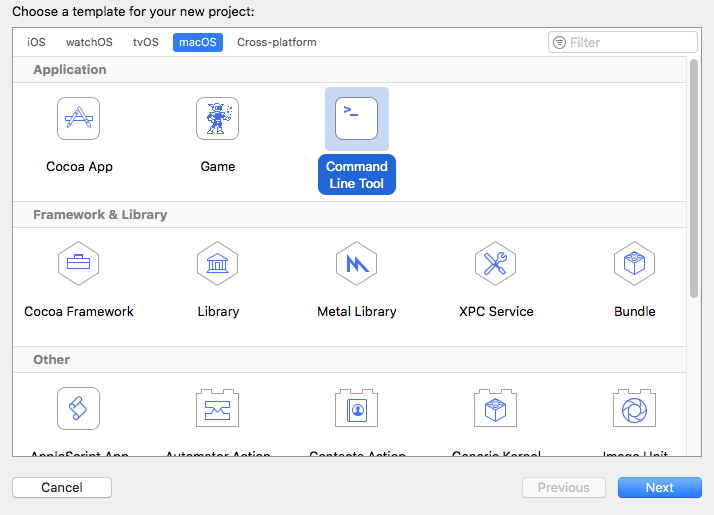
\includegraphics[width=0.7\textwidth]{xcode_images/template.png}
\end{center}\end{center}
\end{frame}
\begin{frame}[label={sec:orge07d780},fragile]{Installation von MCIGraph --- XCode auf MacOS X}
 \begin{itemize}
\item Stellen Sie als Sprache C++ ein:
\end{itemize}
\begin{center}\begin{center}
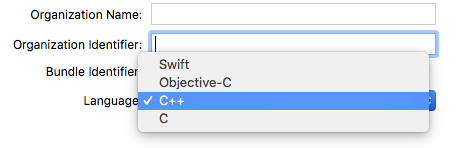
\includegraphics[width=0.5\textwidth]{xcode_images/language.png}
\end{center}\end{center}
\begin{itemize}
\item Führen Sie auf dem Terminal den Befehl {\color{solarizedYellow}\texttt{sdl2-config -{}-cflags} }aus und
kopieren Sie das Ergebnis in die C++ Flags der Build Optionen
\end{itemize}
\begin{center}\begin{center}
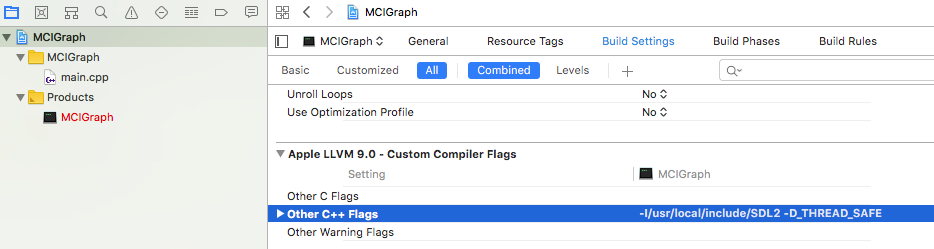
\includegraphics[width=.9\linewidth]{xcode_images/cflags.png}
\end{center}\end{center}
\end{frame}
\begin{frame}[label={sec:orgb4d2bf0},fragile]{Installation von MCIGraph --- XCode auf MacOS X}
 \begin{itemize}
\item Führen Sie auf dem Terminal den Befehl {\color{solarizedYellow}\texttt{sdl2-config -{}-libs} }aus und
kopieren Sie das Ergebnis in die Linker Flags der Build Optionen
\end{itemize}
\begin{center}\begin{center}
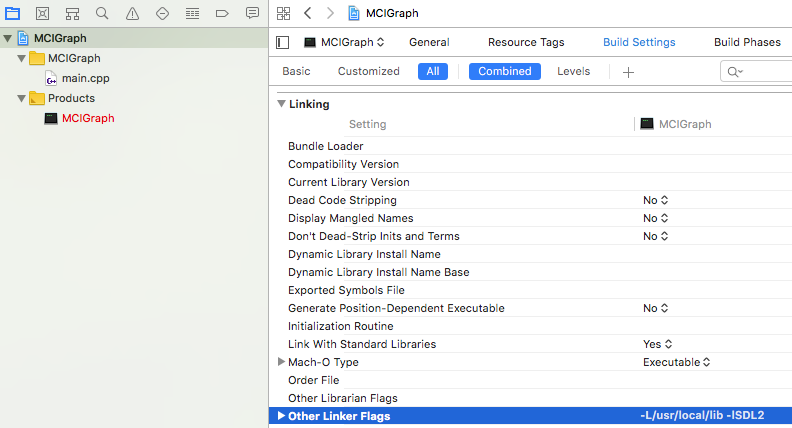
\includegraphics[width=.9\linewidth]{xcode_images/linkerflags.png}
\end{center}\end{center}
\end{frame}
\begin{frame}[label={sec:orgbf187a0},fragile]{Installation von MCIGraph --- XCode auf MacOS X}
 \begin{itemize}
\item Fügen Sie die Datei {\color{solarizedYellow}\texttt{mcigraph.hpp} }aus Sakai ihrem Projekt hinzu:
\end{itemize}
\begin{center}\begin{center}

\includegraphics[width=0.5\textwidth]{xcode_images/addfiles.png}
\end{center}\end{center}
\end{frame}
\begin{frame}[label={sec:org86d3c92},fragile]{Installation von MCIGraph --- Generell}
 \begin{itemize}
\item Laden Sie die für ihr System passenden Bibliotheken von
\url{https://www.libsdl.org/download-2.0.php}
\item Suchen Sie im Internet wie sie ihre Entwicklungsumgebung für SDL2
einrichten können.
\item Laden sie die Datei {\color{solarizedYellow}\texttt{mcigraph.hpp} }von Sakai und speichern sie diese
im selben Verzeichnis wie ihre Quellcodedatei.
\end{itemize}
\end{frame}
\section{Verwendung}
\label{sec:org8345255}
\begin{frame}[label={sec:orgaaa5f04},fragile]{Hello World}
 \begin{block}{Source Code}
\begin{minted}[fontsize=\scriptsize,numberblanklines=false]{c++}
#include "mcigraph.hpp"

int main(int argc, char *argv[]) {
  while (running()) {
    draw_rect(200, 300, 200, 100);
    present();
  }

  return 0;
}
\end{minted}
\end{block}
\begin{block}{Resultat}
\begin{center}\begin{center}

\includegraphics[width=0.25\textwidth]{data/14/80e905-1de5-4f8b-a64b-5545534fed55/screenshot-20170303-163618.png}
\end{center}\end{center}
\end{block}
\end{frame}
\begin{frame}[label={sec:orgd12e695},fragile]{Das verwendete Koordinatensystem}
 \begin{center}\begin{center}
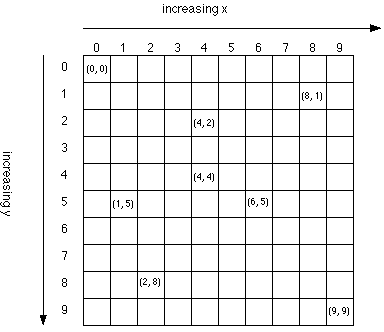
\includegraphics[width=0.7\textwidth]{data/16/2a5cf8-7d19-417f-b610-b412a11366f8/screenshot-20170303-173401.png}
\end{center}\end{center}
Wir haben Koordinaten von {\color{solarizedYellow}\texttt{0} }bis {\color{solarizedYellow}\texttt{1023} }auf der x-Achse und von {\color{solarizedYellow}\texttt{0}}
bis {\color{solarizedYellow}\texttt{767} }in der y-Achse!
\end{frame}
\begin{frame}[label={sec:org2fd1606},fragile]{Zeichne Linie}
 \begin{minted}[fontsize=\scriptsize,numberblanklines=false]{c++}
draw_line(int x1, int y1, int x2, int y2, [int red, int green, int blue])
\end{minted}
\begin{itemize}
\item {\color{solarizedYellow}\texttt{x1} }und {\color{solarizedYellow}\texttt{y1} }: Startkoordinate der Linie
\item {\color{solarizedYellow}\texttt{x2} }und {\color{solarizedYellow}\texttt{y2} }: Endkoordinate der Linie
\item {\color{solarizedYellow}\texttt{red}}, {\color{solarizedYellow}\texttt{green} }und {\color{solarizedYellow}\texttt{blue} }: Optionale Farbe der Linie. Jeder
Farbparameter kann Werte zwischen {\color{solarizedYellow}\texttt{0} }und {\color{solarizedYellow}\texttt{255} }annehmen.
\end{itemize}
\end{frame}
\begin{frame}[label={sec:org0d293c4},fragile]{Zeichne Linie --- Beispiel}
 \begin{minted}[fontsize=\scriptsize,numberblanklines=false]{c++}
#include "mcigraph.hpp"

int main(int argc, char *argv[]) {
  while (running()) {
    draw_line(100, 100, 500, 100, 255, 0, 0);
    draw_line(500, 100, 500, 500, 0, 255, 0);
    draw_line(500, 500, 100, 500, 0, 0, 255);
    draw_line(100, 500, 100, 100, 255, 0, 255);
    present();
  }
  return 0;
}
\end{minted}
\end{frame}
\begin{frame}[label={sec:org50f563b}]{Zeichne Linie --- Resultat}
\begin{center}\begin{center}
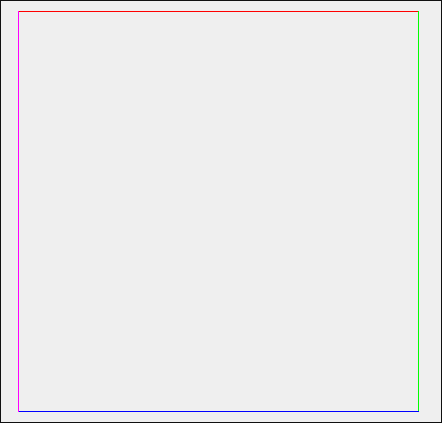
\includegraphics[width=0.8\textwidth]{data/67/54d5a4-1fe1-408b-ba0f-9b700d82c738/screenshot-20170314-211231.png}
\end{center}\end{center}
\end{frame}
\begin{frame}[label={sec:org7cd61b5},fragile]{Zeichne Linie --- Beispiel 2}
 \begin{minted}[fontsize=\scriptsize,numberblanklines=false]{c++}
#include "mcigraph.hpp"
#include <stdlib.h>

int main(int argc, char *argv[]) {
  while (running()) {

    // Zeichne 100 zufällige Linien mit zufälliger Farbe
    for (int i = 0; i < 100; i++) {
      int x1 = rand() % 1024;
      int y1 = rand() % 768;
      int x2 = rand() % 1024;
      int y2 = rand() % 768;
      int red = rand() % 256;
      int green = rand() % 256;
      int blue = rand() % 256;

      draw_line(x1, y1, x2, y2, red, green, blue);
    }
    present();
  }

  return 0;
}
\end{minted}
\end{frame}
\begin{frame}[label={sec:orga40630a}]{Zeichne Linie --- Resultat 2}
\begin{center}\begin{center}
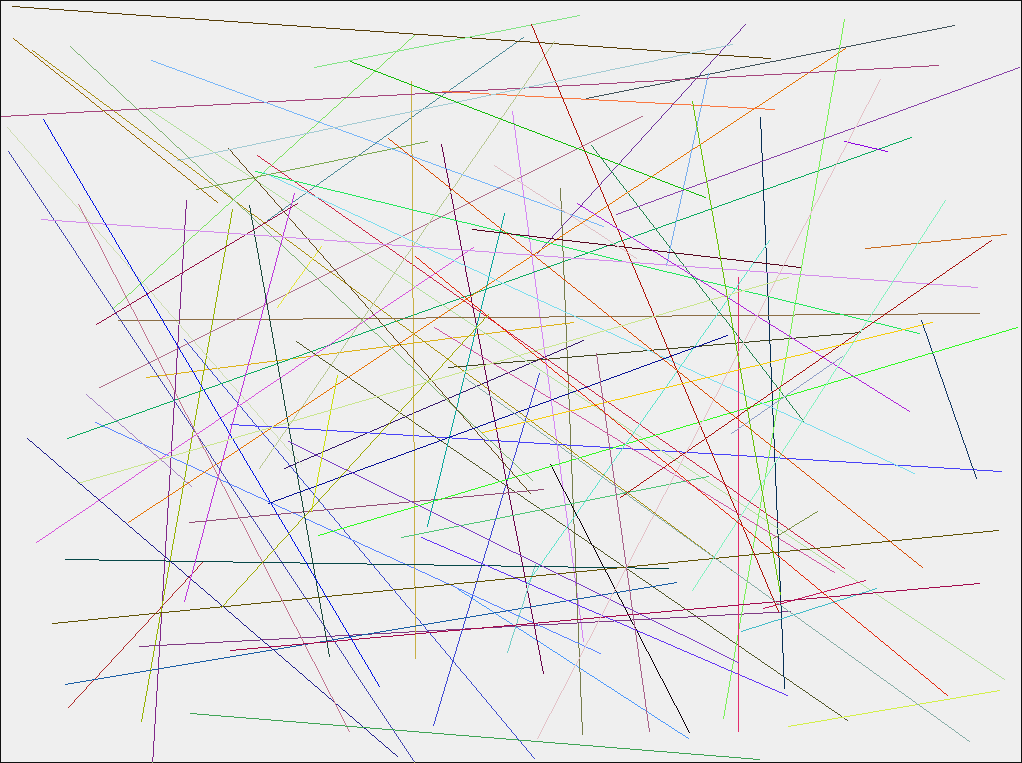
\includegraphics[width=.9\linewidth]{data/db/8df584-32dc-4f72-b1aa-c747e47dac71/screenshot-20170314-212846.png}
\end{center}\end{center}
\end{frame}
\begin{frame}[label={sec:orgda7aaca},fragile]{Zeichne Punkt}
 \begin{minted}[fontsize=\scriptsize,numberblanklines=false]{c++}
draw_point(int x, int y, [int red, int green, int blue])
\end{minted}
\begin{itemize}
\item {\color{solarizedYellow}\texttt{x} }und {\color{solarizedYellow}\texttt{y} }: Koordinaten des Punkts
\item {\color{solarizedYellow}\texttt{red}}, {\color{solarizedYellow}\texttt{green} }und {\color{solarizedYellow}\texttt{blue} }: Optionale Farbe des Punkts. Jeder
Farbparameter kann Werte zwischen {\color{solarizedYellow}\texttt{0} }und {\color{solarizedYellow}\texttt{255} }annehmen.
\end{itemize}
\end{frame}
\begin{frame}[label={sec:orgb5f643d},fragile]{Zeichne Punkt --- Beispiel}
 \begin{minted}[fontsize=\scriptsize,numberblanklines=false]{c++}
#include "mcigraph.hpp"
#include <stdlib.h>

int main(int argc, char *argv[]) {
  while (running()) {

    // Zeichne an jeder Koordinate einen Punkt mit zufälliger Farbe
    for (int x = 0; x < 1024; x++) {
      for (int y = 0; y < 768; y++) {
        int red = rand() % 255;
        int green = rand() % 255;
        int blue = rand() % 255;

        draw_point(x, y, red, green, blue);
      }
    }
    present();
  }

  return 0;
}
\end{minted}
\end{frame}
\begin{frame}[label={sec:org823e30c}]{Zeichne Punkt --- Resultat}
\begin{center}\begin{center}

\includegraphics[width=.9\linewidth]{data/86/91cde7-2819-4d36-b0ad-c8c6603fdd88/screenshot-20170314-214117.png}
\end{center}\end{center}
\end{frame}
\begin{frame}[label={sec:orgbfd5a98},fragile]{Zeichne Rechteck}
 \begin{minted}[fontsize=\scriptsize,numberblanklines=false]{c++}
draw_rect(int x, int y, int width, int height,
          [bool outline, int red, int green, int blue])
\end{minted}
\begin{itemize}
\item {\color{solarizedYellow}\texttt{x} }und {\color{solarizedYellow}\texttt{y} }: Koordinate des linken oberen Punkts
\item {\color{solarizedYellow}\texttt{width} }und {\color{solarizedYellow}\texttt{height} }: Breite und Höhe des Rechtecks in Pixeln
\item {\color{solarizedYellow}\texttt{outline} }: Wenn {\color{solarizedYellow}\texttt{false} }wird ein gefülltes Rechteck gezeichnet
\item {\color{solarizedYellow}\texttt{red}}, {\color{solarizedYellow}\texttt{green} }und {\color{solarizedYellow}\texttt{blue} }: Optionale Farbe des Punkts. Jeder
Farbparameter kann Werte zwischen {\color{solarizedYellow}\texttt{0} }und {\color{solarizedYellow}\texttt{255} }annehmen.
\end{itemize}
\end{frame}
\begin{frame}[label={sec:orgc2e3f34},fragile]{Zeichne Rechteck --- Beispiel}
 \begin{minted}[fontsize=\scriptsize,numberblanklines=false]{c++}
#include "mcigraph.hpp"
#include <stdlib.h>

int main(int argc, char *argv[]) {
  while (running()) {
    // Zeichne 100 zufällige, gefüllte Rechtecke mit zufälliger Farbe
    for (int i = 0; i < 100; i++) {
      int x = rand() % 1024;
      int y = rand() % 768;
      int width = rand() % 1024 - x;
      int height = rand() % 768 - y;
      int red = rand() % 256;
      int green = rand() % 256;
      int blue = rand() % 256;

      draw_rect(x, y, width, height, false, red, green, blue);
    }
    present();
  }

  return 0;
}
\end{minted}
\end{frame}
\begin{frame}[label={sec:orgb376a6f}]{Zeichne Rechteck --- Resultat}
\begin{center}\begin{center}
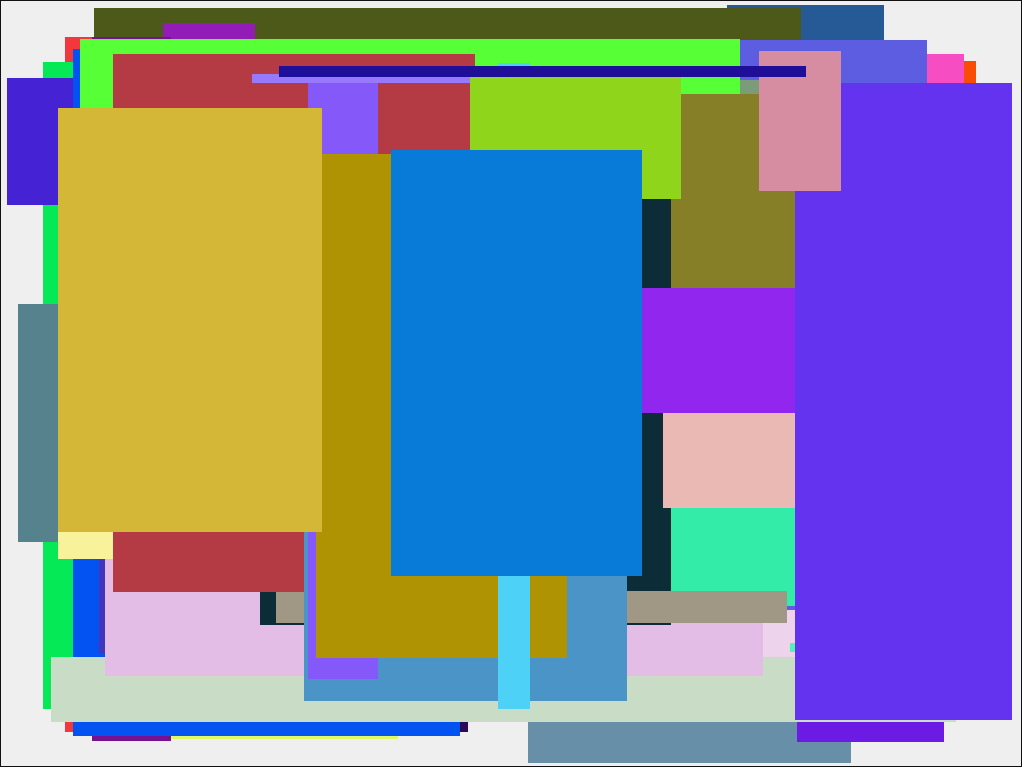
\includegraphics[width=.9\linewidth]{data/74/625dc0-aca5-4a77-8341-259d37547f94/screenshot-20170316-143436.png}
\end{center}\end{center}
\end{frame}
\begin{frame}[label={sec:org1be8bb6},fragile]{Zeige Bild}
 \begin{minted}[fontsize=\scriptsize,numberblanklines=false]{c++}
draw_image(std::string filename, int x, int y)
\end{minted}
\begin{itemize}
\item {\color{solarizedYellow}\texttt{filename} }: Dateiname des Bilds
\item {\color{solarizedYellow}\texttt{x} }und {\color{solarizedYellow}\texttt{y} }: Koordinate des linken oberen Punkts
\end{itemize}
\begin{block}{Mitgelieferte Bilder}
Auf Sakai finden Sie die Datei {\color{solarizedYellow}\texttt{tiles.zip} }welche viele Bilder im
Format \(16 \times 16\) Pixel enthält. Hier eine Auswahl:
\begin{center}\begin{center}
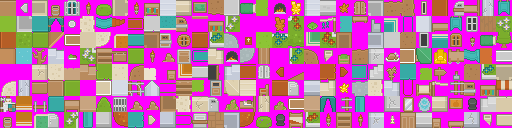
\includegraphics[width=.9\linewidth]{tiles.png}
\end{center}\end{center}
Die Bereiche in Pink werden von MCIGraph transparent dargestellt
\end{block}
\end{frame}
\begin{frame}[label={sec:orgf71d690},fragile]{Zeige Bild --- Beispiel}
 \begin{minted}[fontsize=\scriptsize,numberblanklines=false]{c++}
#include "mcigraph.hpp"
#include <stdlib.h>

int main(int argc, char *argv[]) {
  while (running()) {

    // Fülle das ganze Fenster mit Gras
    for (int x = 0; x < 1024; x += 16) {
      for (int y = 0; y < 768; y += 16) {
        draw_image("grass.bmp", x, y);
      }
    }
    // Setze einen Charakter in die Mitte
    draw_image("character.bmp", 32 * 16, 24 * 16);
    present();
  }

  return 0;
}
\end{minted}
\end{frame}
\begin{frame}[label={sec:org87ac788}]{Zeige Bild --- Resultat}
\begin{center}\begin{center}
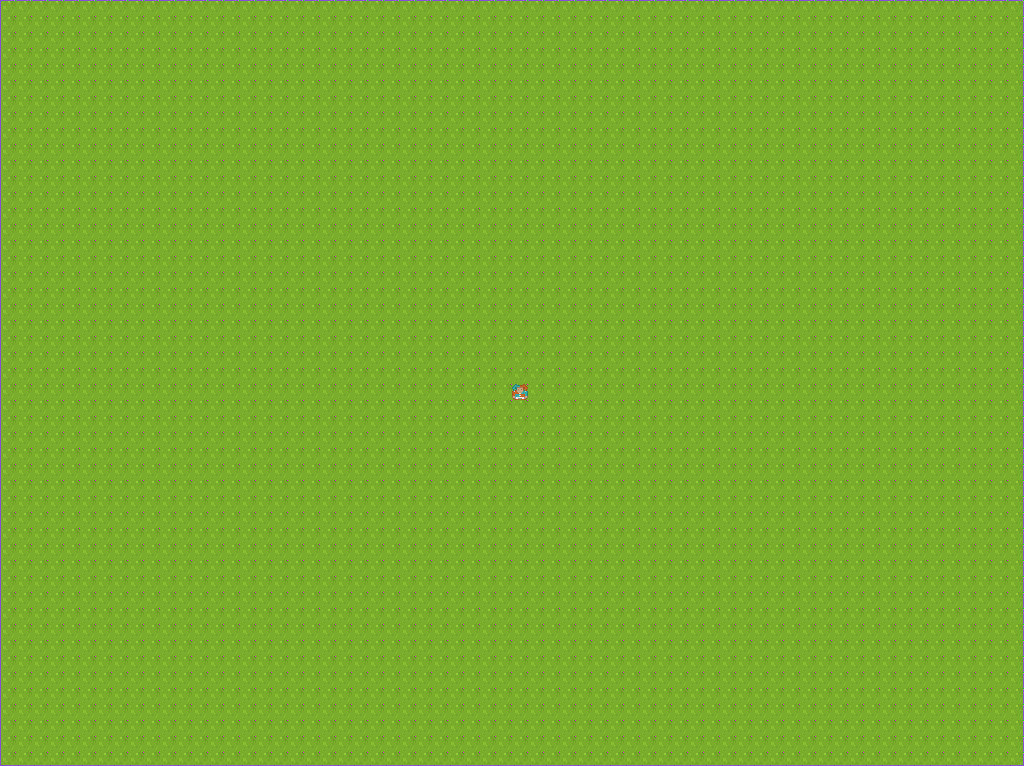
\includegraphics[width=.9\linewidth]{data/34/e7b7d1-9fa0-4cb5-a8fb-42825d77a5f2/screenshot-20170316-144857.png}
\end{center}\end{center}
\end{frame}
\begin{frame}[label={sec:orgdfd4310},fragile]{Frage Tastendrücke ab}
 \begin{minted}[fontsize=\scriptsize,numberblanklines=false]{c++}
bool is_pressed(int keycode)
\end{minted}
\begin{itemize}
\item {\color{solarizedYellow}\texttt{keycode} }: Gibt an welche Taste man abfragen will
\item Die Funktion gibt {\color{solarizedYellow}\texttt{true} }zurück falls die Taste mit {\color{solarizedYellow}\texttt{keycode}}
aktuell gedrückt ist
\end{itemize}
\begin{block}{Keycodes}
\begin{itemize}
\item {\color{solarizedYellow}\texttt{KEY\_LEFT}}, {\color{solarizedYellow}\texttt{KEY\_RIGHT}}, {\color{solarizedYellow}\texttt{KEY\_UP}}, {\color{solarizedYellow}\texttt{KEY\_DOWN}}
\item {\color{solarizedYellow}\texttt{KEY\_SPACE}}
\item {\color{solarizedYellow}\texttt{KEY\_W}}, {\color{solarizedYellow}\texttt{KEY\_S}}, {\color{solarizedYellow}\texttt{KEY\_A}}, {\color{solarizedYellow}\texttt{KEY\_D}}
\item {\color{solarizedYellow}\texttt{KEY\_0} }\ldots{} {\color{solarizedYellow}\texttt{KEY\_9}}
\end{itemize}
\end{block}
\end{frame}
\begin{frame}[label={sec:org826c5dd},fragile]{Frage Tastendrücke ab --- Beispiel}
 \begin{minted}[fontsize=\scriptsize,numberblanklines=false]{c++}
#include "mcigraph.hpp"
#include <stdlib.h>

int main(int argc, char *argv[]) {
  int cx = 32, cy = 24; // aktuelle Position der Spielfigur

  while (running()) {
    for (int x = 0; x < 1024; x += 16) // Fülle das ganze Fenster mit Gras
      for (int y = 0; y < 768; y += 16)
        draw_image("grass.bmp", x, y);

    // Bewege Figur je nach Tastendrücken
    if (is_pressed(KEY_LEFT)) cx--;
    if (is_pressed(KEY_RIGHT)) cx++;
    if (is_pressed(KEY_UP)) cy--;
    if (is_pressed(KEY_DOWN)) cy++;

    draw_image("character.bmp", cx * 16, cy * 16); // Setze die Spielfigur
    present();
  }
  return 0;
}
\end{minted}
\end{frame}
\begin{frame}[label={sec:org48d23b9}]{Frage Tastendrücke ab --- Resultat}
\begin{center}\begin{center}
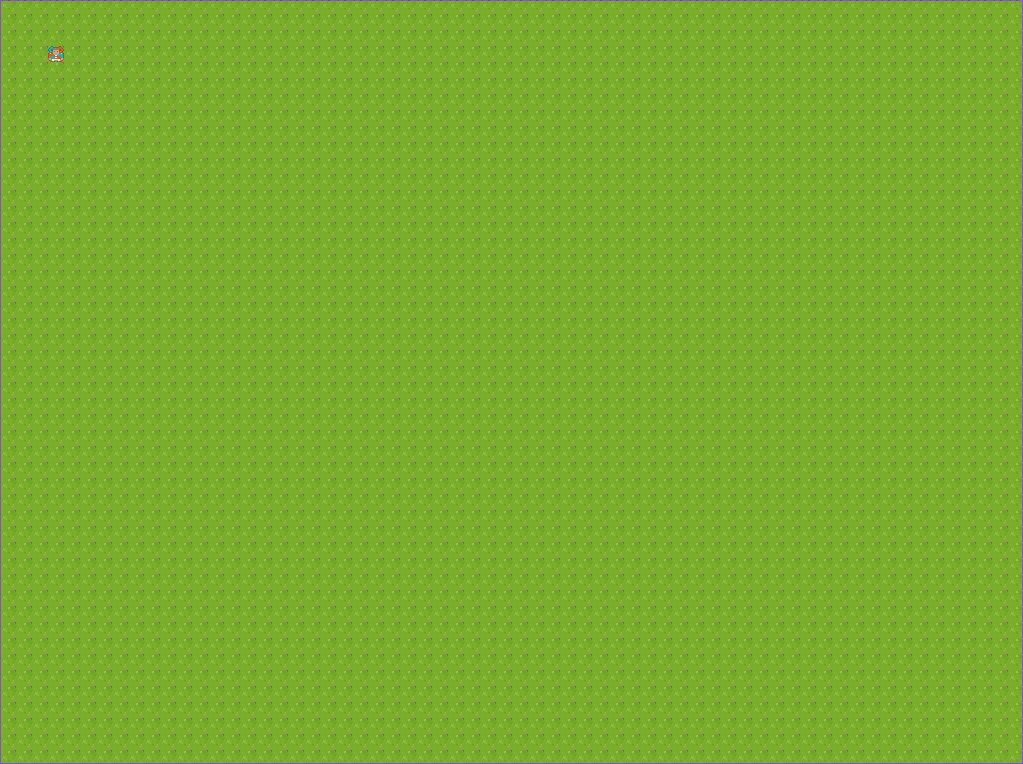
\includegraphics[width=.9\linewidth]{data/d7/603d4d-1dca-45a9-8bea-d56ae35d3f81/screenshot-20170316-150157.png}
\end{center}\end{center}
\end{frame}
\begin{frame}[label={sec:org6ca726b},fragile]{Frage Tastendrücke ab 2}
 Alternativ zu {\color{solarizedYellow}\texttt{is\_pressed} }gibt es auch die Funktion {\color{solarizedYellow}\texttt{was\_pressed(int
keycode)}}. Im Gegensatz zu {\color{solarizedYellow}\texttt{is\_pressed} }liefert diese Funktion nur
{\color{solarizedYellow}\texttt{true} }zurück wenn die Taste seit dem letzten Aufruf erneut gedrückt
wurde. Damit verhält sich diese Funktion eher so wie man es von einer
normalen Tastatureingabe gewöhnt ist.
\begin{block}{Versuch}
Ersetzen Sie alle {\color{solarizedYellow}\texttt{is\_pressed}}-Aufrufe im letzten Programm durch
{\color{solarizedYellow}\texttt{was\_pressed}}- Aufrufe und beobachten Sie das geänderte Verhalten.
\end{block}
\end{frame}
\begin{frame}[label={sec:org89f1ffa},fragile]{Zusätzliche Funktionalität}
 \begin{itemize}
\item Mit {\color{solarizedYellow}\texttt{set\_delay(int x)} }kann eingestellt werden wie schnell das
Programm läuft (wie häufig der Code ausgeführt wird). Ein höherer
Wert führt zu einer langsameren Ausführung.
\end{itemize}
\end{frame}
\begin{frame}[label={sec:orgad2b571}]{Übung}
\begin{enumerate}
\item Erweitern Sie das vorherige Programm so, dass zwei Figuren angezeigt werden
\item Sorgen sie dafür, dass die zweite Figur mit den Tasten WSAD steuerbar ist
\item Verhindern Sie für beide Figuren, dass sie aus dem Spielfeld laufen können
\item Verhindern Sie, dass beide Figuren auf dem selben Feld stehen können
\end{enumerate}
\begin{center}\begin{center}
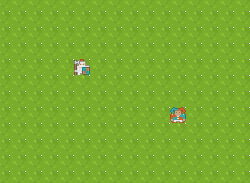
\includegraphics[width=0.5\textwidth]{data/07/5f8661-1d63-4374-98be-36d9b786a222/screenshot-20200228-142923.png}
\end{center}\end{center}
\end{frame}
\end{document}